
%----------------------------------------------------------------------------------------
%	MLA
%----------------------------------------------------------------------------------------

\chapter{MLA Style} 


\section{Formatting the MLA essay}
When setting up your word processor for an MLA-formatted document, use the 
following settings:

\begin{itemize}
\item Set one-inch margins on all sides of the document.
\item Double-space the entire document, including block quotes.
\item In the top left portion of the first page, type your name, instructor's name, course title, and date on separate, double-spaced lines.
\item Include your last name and a page number on each page in the top right corner of the header.
\item Include a centered title on the first page.
\item Indent the first line of each paragraph with a tab set to 1/2 inch.
\end{itemize}

\newpage



When a quotation runs more than four typed lines, use a \hloy{block quote}. A block quote is a freestanding block of quoted words, set apart from the rest of the text. When formatting block quotes in MLA, use the following rules: 

\begin{itemize}
\item Begin the block quote on a new line. 
\item Indent every line of the quote 1 inch from the left margin (this should be two tabs). 
\item Do not use quotation marks around the quoted material. 
\item Place the parenthetical citation \emph{after} the final punctuation of the quoted passage.
\end{itemize}

\newpage
\section{MLA page example}

\bigskip

\begin{tcolorbox}[enhanced,width=4.2in,left=.3in, right=.3in,
   drop fuzzy shadow southeast,
    boxrule=0.4pt,sharp corners,colframe=black!80!black,colback=white!10]

\medskip

{\scriptsize \begin{flushright} Tate 1 \end{flushright}
\begin{doublespacing}
Rufus Tate

Prof. Moon

Writ. 2

9/25/16

\begin{center}Emily Dickenson's Poem \#365 \end{center}
\hspace{1.4em} Emily Dickinson's poem \#365 opens with an unequivocal, affirmative declaration pertaining to the existence of God.  Yet, as the poem progresses, the religious conviction displayed in the opening categorical statement "I Know that He Exists" gradually abates until finally transforming into a frantic consideration of the possibility that the life of faith is but a cruel hoax.  The poem's transition from an unswerving certainty, modeled in the opening line's declarative sentence, to the disconcerting and telling ambiguity of the final stanzas therefore compactly summarizes a loss or crisis of religious faith in the speaker.  
  
\hspace{1.4em} The opening line of the poem, "I know that He exists," reads like a statement of scientific fact.  Rather than proffer a statement of faith (a belief in things unseen), the speaker first envisions the problem of God's existence as something resolvable by the operation of reason.  The speaker's resolute claim that she "know[s]" God exists reveals that the issue has been definitively concluded by way of a previous--though unidentified--process of  reasoning.  The unbroken line and full stop, along with the statement's uncompromising, declarative nature, conspire to give the poem's opening line and its assertion about the existence of God the status of unassailable truth.  

\hspace{1.4em}In the following lines of the first stanza, however, the speaker's lack of any real or tangible evidence for her claim becomes apparent, invalidating the former, putatively empirical, understanding of God's existence.  

\end{doublespacing}}
\bigskip


\end{tcolorbox}

%\vspace*{\fill}
%\begin{center}
%\begin{center}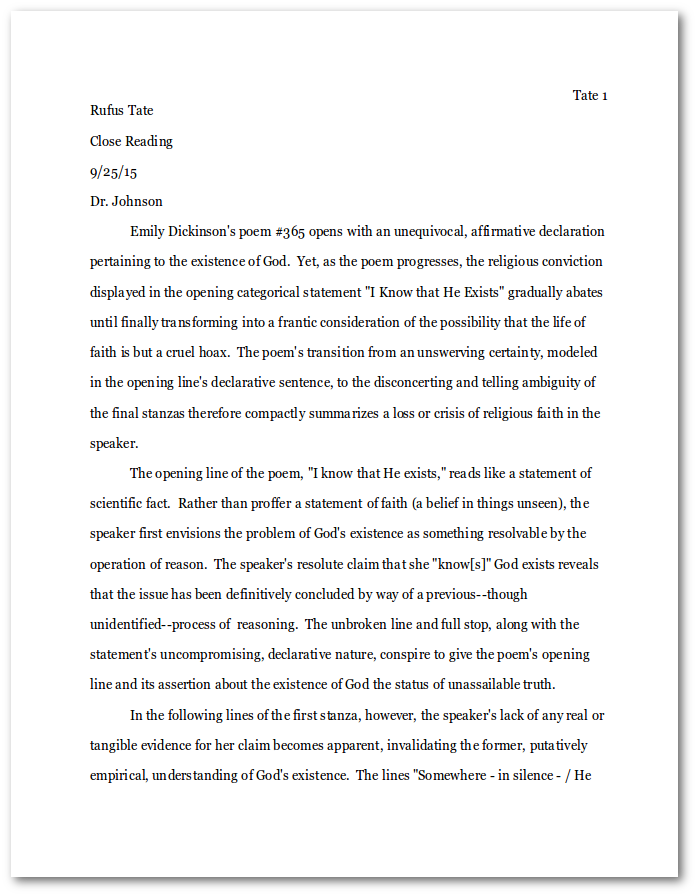
\includegraphics[width=.49\textwidth]{mlastyle}\end{center}
%\end{center}
%\vspace*{\fill}

\newpage
\section{MLA block quote example}
%\vspace*{\fill}
%\begin{center}
%\begin{center}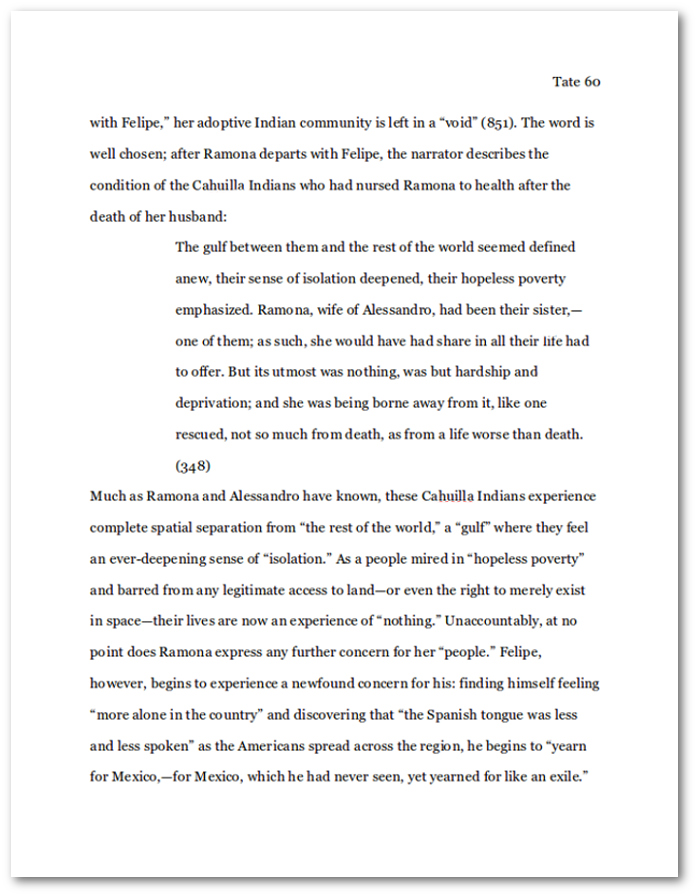
\includegraphics[width=.49\textwidth]{mlablockquote}\end{center}
%\end{center}
%\vspace*{\fill}

\bigskip

\begin{tcolorbox}[enhanced,width=4.2in,left=.35in, right=.35in,
   drop fuzzy shadow southeast,
    boxrule=0.4pt,sharp corners,colframe=black!80!black,colback=white!10]

\medskip

{\scriptsize \begin{flushright} Tate 29 \end{flushright}
\begin{doublespacing}
frequently result in absurdities; an illustration of which may be found in Janie Hinds' 2004 essay on the novel, where she argues the following:
\begin{myenv}The historical Walking Purchase Treaty of 1737, the ‘‘encroachment’’ event alluded to in Edgar Huntly as taking place 30 years before the events of the novel, stipulated that English settlers would own as much territory as they could walk in a day; when the English hired professional runners to cover at least three times as much ground as a person could legitimately cover in walking, the Delaware became understandably hostile, not only about the loss of territory but about the colonists’ trick. (335)\end{myenv}
Hinds here refers to an important moment in the novel when Edgar Huntly explains that the Delaware who formerly lived in the region left due to the “perpetual encroachments of the English colonists” (198). Although Huntly does remark that the departure of the Delaware tribe took place “about thirty years ago,” the event should in no way be confused with the Walking Purchase. Since the novel's setting is almost universally accepted to be in the year 1787, the “encroachments” mentioned by Edgar Huntly must have occurred in, or around, the year 1757—two decades \emph{after} the Walking Purchase. In her attempt to preserve this historical gloss, therefore, Hinds effectively relocates the novel's setting two decades into the past—a claim that contravenes virtually all historical scholarship on the novel and potentially muddles our understanding of the root causes of the native violence in Huntly's narrative. Although the memory of this dishonorable theft of land is undeniably a powerful explanation of the Delaware's revanchist violence within the novel (an argument made by many scholars), we do ourselves a disservice to ignore Brown's plain attempts to have us view his narrative as a statement on “recent incidents.”

\end{doublespacing}}

\bigskip
\smallskip
\smallskip

\end{tcolorbox}



\newpage

\section{In-text citations}
The MLA style uses parenthetical citations to indicate the author and page number of sources. These parenthetical citations take two forms. One form is used when the source you are citing \emph{is named or understood} by your audience. The other form is used when the author being cited is \emph{unknown or unclear}. 

\begin{enumerate}

\item \hloy{Author is named or understood}. \smallskip

In the following sentence the author of the source in question is obvious. Since the author is known to the reader, the parenthetical citation uses \textbf{only the page number} of the source: 

\begin{quote}
According to scholar James Frey, "Each American consumes five pounds of ice cream 
annually" (78).
\end{quote}

\item \hloy{Author is not named or understood}. \smallskip

In the following versions of the sentence, however, the author is not stated:

\begin{quote}
According to one scholar, "Each American consumes five pounds of ice cream 
annually" (Frey 78).
\end{quote}

\noindent Or:
\begin{quote}
Studies have shown that the American people consume an average of five pounds of ice 
cream every year (Frey 78).
\end{quote}

\noindent In the first sentence, the author is referred to only as a generic "scholar." To give the reader information on which scholar is being cited, Frey's name is included in the parenthetical citation. In the second sentence the author describes the report, not its author; as a result, the student has included Frey's name to indicate whose report is being referenced. 

\end{enumerate}

\bigskip

\begin{tcolorbox}[colframe=oyster, coltitle=black, sharp corners, title=\ding{52} In-text citations for media like film or music. ]

For media that has a runtime\textemdash like film, television, or music\textemdash MLA now requires that you cite a timestamp within your in-text citations. Use colons to separate hours, minutes, and seconds. For example:

\begin{itemize}
\item According to Rushmore Academy's headmaster, Max is "probably the worst student" at the school (00:04:04-07).

\smallskip

\item In "Don't Hurt Yourself," Beyoncé proclaims "I am the dragon breathing fire" (01:13-15).
\end{itemize}

\end{tcolorbox}



%----DONE-----------

\section{List of Works Cited}

MLA requires a bibliography at the conclusion of the essay that includes the full 
citation of the sources cited within the essay. In MLA, the bibliography is known as the 
\hloy{Works Cited} page. When setting up a Works Cited page, use the following rules and 
characteristics:

\begin{itemize}
\item Center the words "Works Cited" at the top of the page.
\item Use your last name and the page number on the right side of the page's header.
\item Double space the entries.
\item Alphabetize the entries by the author's last name.
\item If an entry runs more than one typed line, indent the second (and any subsequent) line with a 1/2-inch tab.
\item If two or more works by the same author are used, list the entries alphabetically by title. After the first entry, replace the author's name with three dashes followed by a period.
\end{itemize}
\newpage

\section{Works Cited example}
%\begin{center}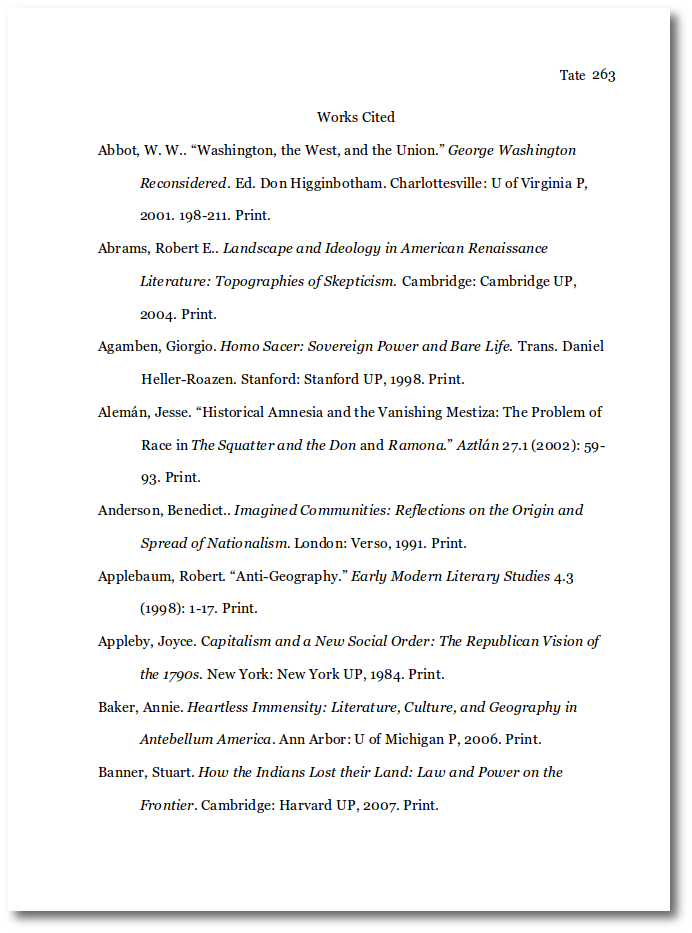
\includegraphics[width=.48\textwidth]{mlaworkscited}\end{center}

\bigskip

\begin{tcolorbox}[enhanced,width=4.2in,left=.3in, right=.3in,
   drop fuzzy shadow southeast,
   halign=flush left,
    boxrule=0.4pt,sharp corners,colframe=black!80!black,colback=white!10]

\medskip

{\scriptsize \begin{flushright} Taylor 12 \end{flushright}

\begin{doublespacing}
\begin{center}Works Cited \end{center}
\hangindent3em{
Abrams, Robert E. \emph{Landscape and Ideology in American Renaissance Literature: Topographies of Skepticism}. Cambridge UP, 2004.}

\hangindent3em{Alemán, Jesse. “Historical Amnesia and the Vanishing Mestiza: The Problem of Race in \emph{The Squatter and the Don} and \emph{Ramona}.” \emph{Aztlán}, vol. 27, no. 1, 2002, pp. 59-93.}

\hangindent3em{Anderson, Benedict. \emph{Imagined Communities: Reflections on the Origin and Spread of Nationalism}. Verso, 1991.}

\hangindent3em{Baas, Robert. “Anti-Geography.” \emph{Early Modern Literary Studies}, vol. 4, no. 3, 1998, pp. 1-17.}

\hangindent3em{Bjorn, Joyce. \emph{Capitalism and a New Social Order: The Republican Vision of the 1790s}. NYU UP, 1984.}

\hangindent3em{Carver, Annie. \emph{Grave Dangers: Spirits and Hauntings in the American Renaissance}. U of Michigan P, 2006.}

\hangindent3em{Graves, Stuart. \emph{How the Indians Lost their Land: Law and Power on the Frontier}. Harvard UP, 2007.}

\hangindent3em{Hill, William. \emph{History of the Blue Ridge}. Dobbs Publishing, 1987.}

\hangindent3em{
- - -. \emph{The Highest Lost Cause: Signal Mountain and the Civil War}. Peach Publishing, 1988.
}

\hangindent3em{
Kleiner, Randy. \emph{Escaping the Redneck Riviera}. Peach Publishing, 1988.
}

\hangindent3em{Linter, Fred. \emph{The Theory of Landscape}. Boston UP, 1999.
}

\hangindent3em{
Zanner, Jeff E. \emph{Language on the Frontier}. Edited by Robert Snooks, Indiana UP, 2012.}

\end{doublespacing}}

\bigskip
\bigskip
\bigskip
\bigskip
\end{tcolorbox}


\newpage

\section{The MLA bibliography}

The eighth edition of the \emph{MLA Handbook}, published in 2016, issued sweeping changes to the formatting of the MLA bibliography. The previous seven editions of the handbook attempted to provide a model citation for every type of source. However, the explosion of internet-based sources and new forms of communication and media made the project of providing guidance on every type of source challenging.  

The new handbook replaces the creation of an ever-growing list of source types with a set of universal guidelines that may be used to formulate a citation for any type of source. These guidelines are referred to as the "core elements."

\section{The MLA core elements}

%\bigskip

%\begin{center}
%\begin{tcolorbox}[colframe=Ahrenge, sharp corners, title=\ding{52} The MLA "core elements"]

%\hangindent1.2cm{
%Author. Title. Title of container (self contained if book), Other contributors (translators or editors), Version (edition), Number (vol. and/or no.), Publisher, Publication Date, Location (pages, paragraphs URL or DOI). 2nd container’s title, Other contributors, Version, Number, Publisher, Publication date, Location, Date of Access (if needed).}

%\end{tcolorbox}
%\end{center}
These core elements are presented in the order they should appear within your bibliography. The proper punctuation that follows each of the core elements is also provided. Thus, you will begin the entry with the author's name, followed by a period. Then the title of the work will be provided, followed by a period. And so on. If one of these core elements does not apply to your source, skip it and move to the next one until you have been through the entire list of elements. The promise of this new approach is that it provides a method for citing any type of source, even those that do not exist yet.

\newpage

\begin{center}
\begin{tcolorbox}[colframe=oyster, coltitle=black, sharp corners, title=\ding{52} The MLA "core elements"]
\begin{itemize} 
{\small
\item Author. 

\item Title. 

\item Title of container (self contained if book), 

\item Other contributors (translators or editors), 

\item Version (edition), 

\item Number (vol. and/or no.), 

\item Publisher, 

\item Publication Date, 

\item Location (pages, paragraphs URL or DOI). 

\smallskip

\rule{8cm}{.1em}

\smallskip

\item 2nd container’s title, 

\item Other contributors, 

\item Version, 

\item Number, 

\item Publisher, 

\item Publication date, 

\item Location, 

\item Date of Access (if needed).
}
\end{itemize}

\end{tcolorbox}
\end{center}


\section{Using the MLA "core elements"}

\subsection{1. Author.}

The first element of a citation is the author's name. Since the MLA bibliography is organized alphabetically by the author's last name, begin your citations with the author's last name, followed by a comma, then the author's first name. If a middle name or initial are supplied, include those after the first name in the entry. Conclude the author element with a period. Often, sources will  have multiple authors. In that case, only the first listed author will use the Last Name, First Name structure. For example: \bigskip

\hangindent1.2cm{
\hl{Taylor, Alan C.} {\emph{A Tour of New Hampshire's Wolf Trees}}. Little and Sons, 1998.
}

\smallskip
 
\hangindent1.2cm{
\hl{Zane, John, Philip Glass and Jane Hinds}. \emph{Recovering the City of Boston}. U of Massachusetts P, 2000.}


\subsection{2. Title of source.}

The title of a source is italicized if it is considered "self-contained" and "independent." Sources that are part of a larger whole, however, are placed in quotation marks. For example, a book is a self-contained and independent source; however, a \emph{chapter in a book} is part of a larger whole. Thus, the title of the book will be italicized while the title of the chapter will appear in quotation marks. Similarly, a television series is an independent whole, so its title will be italicized. However, an episode within the television series is part of the larger program, so its title appears in quotations. For example: \bigskip 

\hangindent1.2cm{
San, Rathanak. \emph{\hl{Escaping Vietnam}}. Peach Publishing, 1988.
}

\smallskip

\hangindent1.2cm{
Taylor, James. "\hl{The Indian Matter of Charles Brockden Brown's Writings.}" \emph{American Literature}, vol. 45, no. 6, 1998, pp. 432-45.} 

\hangindent1.2cm{
"\hl{Say My Name}." \emph{Breaking Bad}, created by Vince Gilligan, performance by Brian Cranston, season 5, episode 7, AMC, 2012.
}

\begin{center}
\begin{tcolorbox}[colframe=oyster, coltitle=black, sharp corners, title=\ding{52} Capitalization of titles in MLA]

MLA has a standardized approach to the capitalization of titles. Regardless of how the title appears on a title page, scholarly journal, or database, use the following information to properly capitalize the title of your source on your Works Cited page:

\medskip
\begin{itemize}
\item Capitalize nouns, pronouns, verbs, adjectives, adverbs, and subordinating conjunctions.

\item Unless they begin the title, do not capitalize articles, prepositions, coordinating conjunctions, or the "to" in infinitive verbs.
\end{itemize}

\end{tcolorbox}
\end{center}


\subsection{3. Title of container,}

Many kinds of sources are smaller parts of larger wholes. MLA refers to these larger wholes as "containers." For example, a chapter is a smaller part of a book. In this sense, the book is the container for the chapter. Similarly, a scholarly article is a smaller part of the scholarly journal that contains it. Newspaper articles, essays in a collection, and television episodes are all contained by a larger context. These containers are italicized in your bibliography. For example, here are the citations for an article in a scholarly journal and a work in a collection of essays:

\bigskip

\hangindent1.2cm{
Taylor, James. "The Indian Matter of Charles Brockden Brown's Writings." \emph{\hl{American Literature}}, vol. 45, no. 6, 1998, pp. 432-45.} \bigskip


\hangindent1.2cm{
Cranston, William. "My Famous Donkey." \emph{\hl{Writings from East Tennessee,}} edited by Jax Ridley, East Tennessee State P, 2011, pp. 77-90.} \bigskip

\noindent Some sources have multiple containers. This is often true for electronic sources. For example, a scholarly article may be contained by both the journal that published it and the academic research database that hosts it online. Consider an article published in the academic database called \href{https://www.jstor.org/}{JSTOR}: \bigskip

\hangindent1.2cm{
Taylor, James. "The Indian Matter of Charles Brockden Brown's Writings." \emph{American Literature}, vol. 45, no. 6, 1998, pp. 432-45. \hl{\emph{JSTOR}, www.jstor.org/stable/8759038475.}} \bigskip

\noindent When citing a source make sure that you represent \emph{every} container so as to truly represent where that source was discovered. 

\subsection{4. Other contributors,}

Your sources will often have a number of other individuals who contributed to the work besides the author(s). You may find sources with one or more of these additional roles:

\begin{itemize}

\item director
\item editor
\item illustrator
\item introducer
\item narrator
\item performer
\item translator
\end{itemize}

\hangindent1.2cm{
Taylor, Alan C. {\emph{A Tour of New Hampshire's Wolf Trees}}. \hl{Edited by Arthur S. Cohen}, Little and Sons, 1998.} \bigskip

\hangindent1.2cm{
Jens, Ryn G. "Morning Glory." \emph{A Runner's Bible,} \hl{translated by Arthur S. Cohen}, Greenwater Press, 1974, pp. 45-58.} \bigskip



\subsection{5. Version,}

Many sources are published in more than one version. The most common version you will encounter in academic research is a new version of a book. Each new version of a book is described as an \textbf{edition}. These versions are numbered in sequential order: 1st edition, 2nd edition, 3rd edition, and so on. There are other kinds of versions, some of which are described below. 

\bigskip 

\hangindent1.2cm{
\emph{The Bible}. \hl{Authorized King James Version}, Oxford UP, 1998.} \bigskip

\hangindent1.2cm{
Smith, John. \emph{Raising Arizona}. \hl{3rd ed.}, Primer Publishing, 1993.} \bigskip

\hangindent1.2cm{
David, Gray. \emph{Blister in the Sun}. \hl{Revised ed.}, Primer Publishing, 1993.} \bigskip

\hangindent1.2cm{
Anderson, Wes. \emph{Rushmore}. 1998. Performance by Bill Murray and Jason Schwartzman, \hl{director's cut}, Buena Vista International, 2017.}\bigskip

\noindent Always ensure that you cite the exact version that you use in your writing. Pagination often differs between editions; versions of a film or other media may vary signifiantly or have additional content. Failing to cite the specific version of a text will lead to confusion and may make your readers feel that you are sloppy or uncaring. 

\subsection{6. Number,}

Many sources are part of a numbered sequence. For the most part you will encounter this in \textbf{journal articles} and \textbf{books that are part of a numbered series}.
 
\bigskip

\begin{itemize}
\item Journal articles are often collected together in volumes and numbered issues: 
\end{itemize}

\hangindent1.2cm{
Taylor, James. "The Indian Matter of Charles Brockden Brown's Writings." \emph{American Literature}, \hl{vol. 45, no. 6}, 1998, pp. 432-45.}\medskip

\begin{itemize}
\item Some journals do not collect issues into numbered volume numbers; instead, they only publish numbered issues:\end{itemize}

\hangindent1.2cm{
Yeti, Smitty. "Genocide in South America." \emph{Journal of Violence}, \hl{no. 7}, 1990, pp. 221-75.}\medskip

\begin{itemize}
\item When books are too large to be published as a single text, they are organized in volumes: 
\end{itemize}

\hangindent1.2cm{
Smith, Jeb. \emph{A History of American Serial Killers}. \hl{Vol. 6}, Samford UP, 2012.}


\subsection{7. Publisher,}

A publisher is the business or organization responsible for bringing a book, article, website, or other type of source to the public. \textbf{Books} will commonly indicate the publisher on the title or copyright pages, which will be the first few pages of the text: \bigskip 

\hangindent1.2cm{
Lund, Frank. \emph{The Gravest of Errors}. \hl{Indiana UP}, 2012.}\bigskip

\noindent \textbf{Websites} or \textbf{blogs} may not have clear indications for the publisher. However, this information is often included in the footer at the bottom of a homepage or on "About" or "Contact" pages: \medskip

\hangindent1.2cm{
Teeter, Graham. "My Time Alone in Vietnam, a Travel Tale." \emph{Narratives from the Edge}, \hl{Society of World Geographers}, www.edgenarratives.com/teeter}. \bigskip

\noindent Television series and films are often created by a large array of producers and companies. However, cite only the organization that had the primary responsibility for production:\bigskip 

\hangindent1.2cm{
Anderson, Wes. \emph{Rushmore}. Performance by Bill Murray and Jason Schwartzman, \hl{Buena Vista International}, 1998.}\bigskip



\begin{center}
\begin{tcolorbox}[colframe=oyster, coltitle=black, sharp corners, title=\ding{52} When \emph{not} to include the publisher]
The MLA stylebook explains several situations where a publisher's name is \emph{not} required in the citation: 

\begin{itemize}
\item A periodical (academic journal, newspaper, magazine, etc.)
\item A work published by its author.
\item A website whose title is essentially the name of the publisher.
\item A website that does not help produce the source, only host it (academic database, youtube, etc.)
\end{itemize}

\medskip

Be careful, however, to include things like the electronic database name or platforms like youtube as \textbf{containers}, described above.


\end{tcolorbox}
\end{center}




\subsection{8. Publication date,}

Most sources appropriate for academic research will clearly disclose the date, or dates, of publication. This information will often appear in the front matter of books or journals, or in the masthead of newspapers. 

Online sources, however, present a problem. Sometimes it is unclear when an online source was published. Other times the online source may be a digital version of a print source which may have been published at a different time. 

When a source has more than one publication date, cite only the version that you are using in your own writing. For example, if you are citing a newspaper article you read online, you should cite the date disclosed on the online version, not the corresponding print version. Failing to do this may cause problems if the online version was edited after the newspaper went to print.

\subsection{9. Location,}

The location of a source largely refers to a source's \textbf{page number, or numbers}. However, many types of sources do not have page numbers. A web page's location, for example, is a \textbf{URL}. And a painting or statue's location would be the \textbf{physical location} of the museum where you viewed it in person. 

\begin{itemize}
\item A chapter in a book:
\end{itemize}

\hangindent1.2cm{
Tate, Justin. "Ordering Wine in Paris." \emph{An American's Guide to French Cuisine}, U of Tennessee P, 1989, \hl{pp. 45-61}}. \bigskip

\noindent If the source is only on a single page, use p. rather than pp. to indicate the page number.

\begin{itemize}
\item A website:
\end{itemize}

\hangindent1.2cm{
Grisham, Wyatt. "A Soccer Mom's Lament." \emph{Sports and Parenting}, 28 Oct. 2017, \hl{www.sandp.org/soccermomslament}}. \bigskip

\noindent URLs can be challenging to present because of their length or mutable nature. If possible, use what is known as a permalink\textemdash a permanent URL associated with online content. These permalinks will not change over time. You may also find online content with a DOI, a digital object identifier. You may cite this DOI in place of a URL. If a URL is too long to include in your bibliography, you may use a shortened version of the URL by citing the domain name of the source. For example: www.nytimes.com.


\begin{center}
\begin{tcolorbox}[colframe=oyster, coltitle=black, sharp corners, title=\ding{52} Note]

Previous versions of the MLA handbook required that the city of publication be included for the citation of books. This is no longer required. 


\end{tcolorbox}
\end{center}




\begin{itemize}
\item A material object or work of art:
\end{itemize}

\hangindent1.2cm{
Wayins, Brill. \emph{Lone Pine Tree}. 2001, \hl{Hood Museum of Art, Hanover}.

\section{The MLA bibliography}

While the new edition of the MLA Handbook largely dispenses with specific templates for making citations, I have retained the following examples for this edition of the \emph{Open Handbook}. Although the objective of the MLA "core elements" is to dispense totally with standardized templates, I find that these examples are still a helpful guide, especially for students who lack experience with this style of citation. 

The following section provides examples for citing sources that are commonly found in academic writing. The various forms have been organized into sections on \textbf{books}, \textbf{periodicals}, \textbf{electronic sources}, and \textbf{other types of sources} that are less common.


\section{Book forms}

\subsection{A book by one author}

\hangindent1.2cm{
Taylor, Herman. {\emph{A Tale of One City}}. Little and Sons, 1998.
}


\subsection{Two or more works by the same author(s)}

\hangindent1.2cm{
San, Rathanak. \emph{Escaping Vietnam}. Peach Publishing, 1988.}

\medskip

\hangindent1.2cm{
\noindent- - -. \emph{The Golden Triangle}. Gray and Long, 1999.}

\medskip

\begin{itemize}\item If you cite two works by the same author, use the author's first and last name in the first instance. Use three dashes followed by a period in place of the author's name for any additional works. Place the works in alphabetical order using the first important word in the title.\end{itemize}

\subsection{Two or three authors}


\hangindent1cm{
Roberts, John, Philip Glass and Jane Hinds. \emph{Recovering the City of Boston}. U of Massachusetts P, 2000.}

\begin{itemize}\item Cite the first author using the typical Last Name, First Name format. For each subsequent author, use First Name Last Name.\end{itemize}

\subsection{Four or more authors}


\hangindent1.2cm{
Bankston, Jonathan, et al. \emph{On Barns}. Woodcraft Publishing, 2013.}

\begin{itemize}\item If a work has four or more authors, you may give the first author's name and then replace the other authors with the Latin term "et al," which means "and others." \end{itemize}

\subsection{A book with an editor}
\hangindent1.2cm{
James, Henry. \emph{Portrait of a Lady}. Edited by Leon Edel, Houghton, 1963.}

\begin{itemize}\item If a work has multiple editors, use "Editors" followed by the editors' names in the order they are listed in the source. \end{itemize}


\subsection{An edition (other than the first)}
\hangindent1.2cm{
Thompson, Fred. \emph{Why I Fight}. 3rd ed., Vanity Publications, 2000.}

\subsection{A republished book}

\hangindent1.2cm{
James, Esther. \emph{My Life}. 1946. Random House, 2001.}

\begin{itemize}\item A \textbf{republished book} is one that was previously published in a different form, perhaps even from a different publisher. For books of this kind, indicate the original year of publication after the title. \end{itemize}

\subsection{Corporate author (written by organization or government)}


\hangindent1.2cm{
John Bigam Society. \emph{The Religions of Kenya}. Nairobi Publishing, 2000.}

\medskip 

\hangindent1.2cm{
\noindent United States, Department of Transportation. \emph{State Highway Signage Regulations}. Government Publishing Office, 2002.}

\begin{itemize}\item If the author of a work is a government or institution, use the name of that organization in place of the author. If the text is the publication of a government, include the name of the department or agency. \end{itemize}

\subsection{An anthology}
\hangindent1.2cm{
Foner, Eric, editor. \emph{An American Voice: A Collection of America's Finest} \emph{Essays}. McKinley and Smith, 2011.}

\subsection{Work in an anthology or collection of essays}
\hangindent1.2cm{
Graves, Thomas. "The History of our National Anthem." \emph{An American Voice: A Collection of America's Finest Essays,} edited by Eric Foner, McKinley and Smith, 2011, pp. 20-41.}

\subsection{No author or editor}

\hangindent1.2cm{
\emph{A Guide to Boston}. Beantown Publishing, 2000.}

\subsection{Forward, introduction, preface, or afterward}

\hangindent1.2cm
{Knox, John. Introduction. \emph{The Life of James}, by Elders Johnson, Random House, 2009, pp. 1-8.}



\subsection{A book with a translator} 
\hangindent1.2cm{
McDougle, Astrid. \emph{The Basics of Gaelic}. Translated by Paddy Maloney, Vintage, 1990.}

\subsection{Multivolume work}

\hangindent1.2cm{Graves, Johanna. \emph{Ronald Reagan and the Iran-Contra Affair}. Vol. 7, Greenstalk Publishers, 1988.}

\subsection{Book in a series}


\hangindent1.2cm{
Smith, Rod. \emph{American Economic Expansion in the Nineteenth Century}. Edited by Andrew Stills, Alfred A. Knopf, 1988. \hl{History of American Economic Development.}}

\begin{itemize}\item Occasionally, a press will publish a series of books about a single topic. If your source is a book in a published series, indicate the name of the series at the conclusion of the citation. \end{itemize}

\subsection{Dictionary or encyclopedia entry}

\hangindent1.2cm{
"Suzerian." \emph{Merriam-Webster's Collegiate Dictionary}. 10th ed., 2008.}

\begin{itemize}\item If you are citing an entry from a reference text like a dictionary or encyclopedia that is organized alphabetically, you do not need to indicate the page number.\end{itemize}

\subsection{Sacred text}

\hangindent1.2cm{
\emph{The Bible}. \hl{Authorized King James Version}, Oxford UP, 1998.} \bigskip

\begin{itemize}\item If you are citing a particular edition of a sacred text, such as the Bible, Koran, or Torah, include that information.\end{itemize}


\subsection{Book with title within the title}


\hangindent1.2cm{
Hixson, Fred. \emph{On Cormac McCarthy's }Blood Meridian. Plainspeak P, 2000.}

\begin{itemize}\item If a book title contains the title of another book or article, remove the italics to indicate the title
of the other work.\end{itemize}
%--------------------------------------------------------------------------------------------
%Periodicals
%-------------------------------------------------------------------------------------------


\section{Periodical forms}

\subsection{Article in a scholarly journal with volume and issue numbers}
\hangindent1.2cm{
Taylor, James. "The Indian Matter of Charles Brockden Brown's \emph{Edgar Huntly}." \emph{American Literature}, vol. 45, no. 6, 1998, pp. 432-45.}

\subsection{Article in a scholarly journal that only numbers issues}
\hangindent1.2cm{
Johnston, Johanna. "A Reading of \emph{Moby Dick}." \emph{North Dakota Quarterly}, no. 45, 1978, pp. 45-56.}


\subsection{Article with a title in the title}
\hangindent1.2cm{
Glastonbery, Wes. "On Teaching \emph{Blood Meridian}." \emph{The Journal of College Writing}, vol. 4, no. 5, 2011.}

\begin{itemize}\item If an article's title contains the title of another text, add italics to internal title.\end{itemize}

\subsection{Article in a newspaper}
\hangindent1.2cm{
McKinley, Robert. "Cat Saved from Dog." \emph{The New York Times}, 7 Oct. 2011, p. B2.}

\begin{itemize}\item When an article appears on nonconsecutive pages, indicate the page where article begins 
then use a "+" sign. \end{itemize}

\subsection{Letter to the editor of a newspaper}
\hangindent1.2cm{
Johnson, Smitty. "Reduce our Property Taxes." Letter, \emph{Henniker Telegraph}, 14 Oct. 2013, p. A2} 

\subsection{A review}
\hangindent1.2cm{
Smith, James. Review of \emph{The Orchard Revival}, by Cormac Freedman. \emph{Oregon Magazine}, 23 Oct. 2011, pp. 34-36.} 

\begin{itemize}
\item If the review has a title, include it in quotations after the author's name.
\end{itemize}

\subsection{An unsigned article in a newspaper}
\hangindent1.2cm{
"A Walk Down Nostalgia Lane." \emph{Chicago Sun}, 28 Oct. 2013, p. B6.}

\subsection{Article in a magazine}
\hangindent1.2cm{
Smith, Jim. "Remembering Tony." \emph{The New Yorker}, Jan. 2010, pp. 12-18.}


%--------------------------------------------------------------------
\section{Online sources}

\begin{center}
\begin{tcolorbox}[colframe=oyster, coltitle=black, sharp corners, title=\ding{52} URLs \& DOIs]

Include the address of any content that you find online.\smallskip

\begin{itemize}
\item When possible, use a "stable url" or "permalink" for this purpose. This address will never change and will allow others to find the content easily. 

\item Some online sources have what is known as a Digital Object Identifier, or DOI. If the source has a DOI, use it in place of a URL.

\item When using a URL, remove the "http://" or "https://" that precedes the address. Instead, begin your url with "www."

\item If a URL is too long to include in your bibliography, you may use a shortened version of the url by citing the domain name of the source. For example: www.nytimes.com.
\end{itemize}

\end{tcolorbox}
\end{center}

\subsection{Article in an online database}

\hangindent1.2cm{
Taylor, Abel. "\emph{Moby Dick} and the Cold War." \emph{American Literature}, vol. 45, no. 6, 2010, pp. 45-57. \emph{JSTOR}, www.jstor.org/stable/ 785463258.}

\begin{itemize}\item Cite the source as you would a print article then include the database name, stable url, or DOI (Digital Object Identifier). \end{itemize}

\subsection{A website as a whole} 
\hangindent1.2cm{
Zimmerman, Constantine. \emph{The Moose Report}. New Hampshire Hiking Club, www.moosereport.org.}


\subsection{A work from a website}
\hangindent1.2cm{
Reagan, John. "The Judo Champion Parent." \emph{Parenthood Online}. 11 Oct. 2011, www.parenthoodonline.org/judo.}


\subsection{Article in an online scholarly journal}
\hangindent1.2cm{
Nelson, Grady. "Electronic Literature Comes of Age." \emph{e-Lit Quarterly}, no. 2, 2012, pp. 45-60. www.elit.org/2/2012/grady.pdf.}

\subsection{Article in an online newspaper}
\hangindent1.2cm{
Taylor, Robert C. "Harvesting Undersea Sponges." \emph{New York Times}, 23 Nov. 2000, www.nytimes.com/2000/11/23/us/sponges.}


\subsection{Article in an online magazine}
\hangindent1.2cm{
James, Brian Taylor. "The New War on Terror." \emph{Foreign Affairs Monthly}, Errata Publishing, 2 Oct. 2009, www.famonthly.org /2009/10/james-terror.}



%Online editorial
%Online film review

\subsection{Email}

\hangindent1.2cm{
Cooledge, John. "My Election Thoughts." Received by Mel Smith, 12 Nov. 2012.}

\begin{itemize}
\item For an email message, use the subject line of the email as the title. Indicate the person, or persons, who received the email after the title and the date it was sent.
\end{itemize}


%Posting from an online discussion board

\subsection{Article from an online reference work, such as Wikipedia}
\hangindent1.2cm{
"Al-Qaeda." \emph{Wikipedia}. Wikimedia Foundation, 25 Aug. 2017, https://en.wikipedia.org/wiki/Al-Qaeda.}



\subsection{Podcast:}
\hangindent1.2cm{
Zeender, Nathan, James Spenser, and Michael Tonsmeire. "Dark Lagers." \emph{Basic Brewing Radio}, 31 Jan. 2013, http://traffic. libsyn.com/basicbrewing/bbr01-31-13darklagers.mp3.}

\section{Other types of sources}

\subsection{A dissertation}
\hangindent1.2cm{
Redburn, Marcus. "A Study of Melville's Aesthetics." Dissertation, Boston University, 1978.}

\subsection{Artwork}
\hangindent1.2cm{
Freeman, Dianna. \emph{Still Life 7}. 2009, Hunter Museum of Art, Chattanooga.}

\begin{itemize}\item For a work of art with no title, include a description of the medium after the author's name. For example: photograph, oil on canvas, watercolor, mixed media. \end{itemize}

\subsection{Film or video clip}
\hangindent1.2cm{
Anderson, Wes, director. \emph{Rushmore}. Buena Vista International, 1998.}\bigskip

\noindent Anderson, Wes, director. \emph{Rushmore}. \hl{Performance by Bill Murray}, Buena Vista International, 1998.}\bigskip

\begin{itemize}\item If the focus of your writing is on a particular performer rather than the film as a whole, include the lead performers in the film after the director. \end{itemize}


%Broadcast interview
%Published interview
%Unpublished letter
%Published letter
%Map or chart
%Musical score
%Sound recording
%Oral presentation
%Paper from a conference
%Performance
%Television or radio program
%Pamphlet, brochure, or press release
%Legal source
%A digital file, such as .mp3, .pdf, etc.

%----------------------------------------------------------------------------------------
% END OF SECTION
%----------------------------------------------------------------------------------------